\chapter{Resultados experimentales}\label{sec:resultados-experimentales}

Los resultados responden primero cómo se construye y se compara Top-\(k\), y después qué cambia al activarlo por margen. Se conservan separados el archivo de características, el panel online y los pilotos físicos. Las tablas generadas para esta revisión se vinculan con 124 fuentes mediante hashes y no añaden ajustes ni mediciones.

\section{P1: del descriptor individual a la concatenación}\label{sec:resultados-fase1}
El benchmark consolidado compara Individual, Completa, Top-\(k\), GFS y Homogénea sobre seis datasets y dos clasificadores. Individual designa la mejor alternativa seleccionada internamente, no el máximo externo de todos los descriptores. El Top-\(k\) de esta primera tabla hereda su tamaño del control GFS; su nombre no significa Top-4 fijo.

\begin{resulttable}
\centering\fontsize{9}{11}\selectfont\setlength{\tabcolsep}{3.6pt}
\caption{Macro-F1 externo de las cinco estrategias con la biblioteca de 21 descriptores. Media y desviación estándar entre particiones; Outex tiene un único split. El máximo de cada fila se destaca sin implicar significancia estadística.}
\label{tab:resultados-confirmatorios}
\textbf{Panel A: macro-F1 externo}\par\smallskip
\begin{tabular}{@{}llccccc@{}}
\toprule
Dataset & Clasif. & Individual & Completa & Top-$k$ & GFS & Homogénea \\
\midrule
DTD & SVM & $0{,}8426\,\pm\,0{,}0109$ & $0{,}8629\,\pm\,0{,}0080$ & $0{,}8684\,\pm\,0{,}0080$ & $\mathbf{0{,}8694}\,\pm\,0{,}0096$ & $0{,}8606\,\pm\,0{,}0086$ \\
DTD & ResMLP & $0{,}8373\,\pm\,0{,}0089$ & $0{,}8608\,\pm\,0{,}0100$ & $0{,}8648\,\pm\,0{,}0084$ & $\mathbf{0{,}8660}\,\pm\,0{,}0095$ & $0{,}8611\,\pm\,0{,}0060$ \\
FMD & SVM & $0{,}9726\,\pm\,0{,}0150$ & $0{,}9644\,\pm\,0{,}0174$ & $\mathbf{0{,}9820}\,\pm\,0{,}0105$ & $0{,}9766\,\pm\,0{,}0135$ & $0{,}9789\,\pm\,0{,}0122$ \\
FMD & ResMLP & $0{,}9690\,\pm\,0{,}0133$ & $0{,}9518\,\pm\,0{,}0203$ & $0{,}9753\,\pm\,0{,}0140$ & $\mathbf{0{,}9783}\,\pm\,0{,}0123$ & $0{,}9773\,\pm\,0{,}0109$ \\
CUReT & SVM & $0{,}9948\,\pm\,0{,}0028$ & $\mathbf{0{,}9989}\,\pm\,0{,}0015$ & $0{,}9989\,\pm\,0{,}0010$ & $0{,}9988\,\pm\,0{,}0008$ & $0{,}9989\,\pm\,0{,}0010$ \\
CUReT & ResMLP & $0{,}9971\,\pm\,0{,}0030$ & $\mathbf{0{,}9993}\,\pm\,0{,}0010$ & $0{,}9986\,\pm\,0{,}0015$ & $0{,}9980\,\pm\,0{,}0013$ & $0{,}9982\,\pm\,0{,}0015$ \\
Outex & SVM & $0{,}9066$ & $\mathbf{0{,}9674}$ & $0{,}9441$ & $0{,}9610$ & $0{,}9307$ \\
Outex & ResMLP & $0{,}9476$ & $0{,}9537$ & $0{,}9607$ & $\mathbf{0{,}9715}$ & $0{,}9306$ \\
\bottomrule
\end{tabular}

\par\medskip\textbf{Panel B: descriptor Individual seleccionado}\par\smallskip
\label{tab:individual-identidad}
\begin{tabular}{@{}lll@{}}
\toprule
Dataset & Clasificador & Descriptor (frecuencia) \\
\midrule
DTD & SVM & SigLIP-B (8/10); DINOv2-L (2/10) \\
DTD & ResMLP & SigLIP-B (10/10) \\
FMD & SVM & SigLIP-B (15/15) \\
FMD & ResMLP & SigLIP-B (15/15) \\
CUReT & SVM & DINOv2-L (2/2) \\
CUReT & ResMLP & DINOv2-S (1/2); DINOv2-L (1/2) \\
Outex & SVM & DINOv2-L (1/1) \\
Outex & ResMLP & N-gramas + SVD (1/1) \\
\bottomrule
\end{tabular}
\par\smallskip{\footnotesize Frecuencias de selección interna; cuando cambia el descriptor, la media del panel A reúne esas elecciones.}
\end{resulttable}
\FloatBarrier

\begin{resulttable}
\centering\fontsize{8}{10}\selectfont\setlength{\tabcolsep}{3.0pt}
\caption{Dimensión media de las representaciones usadas en la evaluación externa con 22 descriptores.}
\label{tab:dimensiones}
\begin{tabular}{@{}llrrrrr@{}}
\toprule
Dataset & Clasif. & Individual & Completa & Top-$k$ & GFS & Homogénea \\
\midrule
DTD & SVM & $819{,}2$ & $20652{,}0$ & $4480{,}0$ & $5390{,}4$ & $2496{,}0$ \\
DTD & ResMLP & $768{,}0$ & $20652{,}0$ & $4211{,}2$ & $4626{,}4$ & $2598{,}4$ \\
FMD & SVM & $768{,}0$ & $20652{,}0$ & $2969{,}6$ & $2687{,}5$ & $2338{,}1$ \\
FMD & ResMLP & $768{,}0$ & $20652{,}0$ & $3404{,}8$ & $3077{,}5$ & $2218{,}7$ \\
CUReT & SVM & $1024{,}0$ & $20652{,}0$ & $3328{,}0$ & $4402{,}0$ & $2944{,}0$ \\
CUReT & ResMLP & $704{,}0$ & $20652{,}0$ & $2176{,}0$ & $2880{,}0$ & $1856{,}0$ \\
Outex & SVM & $1024{,}0$ & $20652{,}0$ & $7808{,}0$ & $6784{,}0$ & $3712{,}0$ \\
Outex & ResMLP & $256{,}0$ & $20652{,}0$ & $6016{,}0$ & $3346{,}0$ & $2176{,}0$ \\
Soil & SVM & $768{,}0$ & $20652{,}0$ & $4898{,}1$ & $3709{,}9$ & $2184{,}5$ \\
Soil & ResMLP & $768{,}0$ & $20652{,}0$ & $5529{,}6$ & $4415{,}6$ & $2235{,}7$ \\
KTH-TIPS2-b & SVM & $832{,}0$ & $20652{,}0$ & $1280{,}0$ & $960{,}0$ & $960{,}0$ \\
KTH-TIPS2-b & ResMLP & $672{,}0$ & $20652{,}0$ & $1600{,}0$ & $1440{,}0$ & $928{,}0$ \\
\bottomrule
\end{tabular}
\par\smallskip{\footnotesize Completa tiene siempre 20.652 coordenadas; las otras estrategias pueden elegir subconjuntos distintos entre particiones.}
\end{resulttable}
\FloatBarrier


Las medias muestran que una concatenación puede mejorar al mejor individual seleccionado, pero añadir indiscriminadamente bloques también puede empeorar. En FMD/SVM, Completa registra aproximadamente 0,9647, frente a 0,9726 de Individual y 0,9820 del Top-\(k\) del control. En Outex/SVM, en cambio, Completa alcanza aproximadamente 0,9656. Las diferencias entre datasets impiden definir una regla uniforme a partir del número de bloques.

La dimensión seleccionada y la calidad se reportan conjuntamente. La reducción de entrada al clasificador es informativa para almacenamiento y ajuste, pero no determina qué extractores dominan el tiempo de una consulta. Los contrastes del benchmark estático y su sensibilidad sin KTH se conservan en el Anexo~\ref{app:resultados-adicionales}. Su alcance no se extiende a los tamaños fijos nuevos por un cambio de etiqueta.

\section{Barrido de k y justificación del caso Top-4}
La reconstrucción del barrido verifica 47 condiciones para cada tamaño de uno a 21 y cada clasificador. Las Tablas~\ref{tab:tm-curva}--\ref{tab:tm-top4-resmlp} y la Figura~\ref{fig:tm-curve} describen ese archivo ampliado. El README inicial del barrido corresponde a menos condiciones y no sustituye sus CSV ampliados.

\begin{table}[!htbp]\centering
\fontsize{9}{11}\selectfont\setlength{\tabcolsep}{4pt}
\caption{Barrido exploratorio ampliado: medias equiponderadas de seis datasets, con 47 condiciones por tamaño y clasificador.}\label{tab:tm-curva}
\begin{tabular}{@{}lrrr@{}}\toprule
k & Macro-F1 SVM & Macro-F1 ResMLP & \% dimensiones SVM\\\midrule
1 & 0,917448 & 0,917119 & 4,28\\
2 & 0,929892 & 0,932352 & 8,37\\
3 & 0,933921 & 0,933727 & 11,70\\
4 & 0,936554 & 0,933077 & 15,42\\
5 & 0,934857 & 0,935195 & 19,02\\
10 & 0,936764 & 0,933165 & 45,17\\
21 & 0,935616 & 0,929877 & 100,00\\
\bottomrule\end{tabular}
\par\smallskip\begin{minipage}{0.98\textwidth}\footnotesize La referencia dimensional son los 21 bloques del barrido, sin N-gramas. El máximo observado no es un tamaño óptimo confirmado.\end{minipage}
\end{table}

\begin{figure}[!htbp]\centering
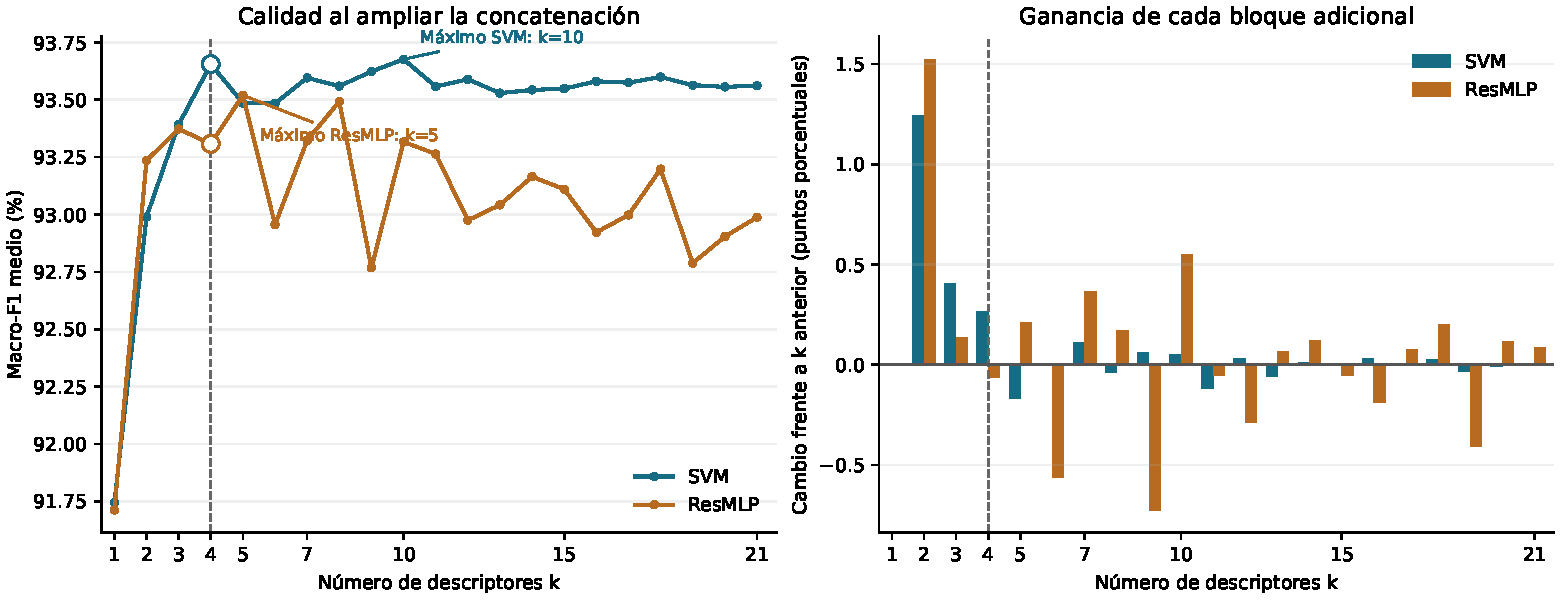
\includegraphics[width=\textwidth]{generated_topk_progression/ganancias_k.pdf}
\caption[Calidad y ganancia marginal al aumentar el número de descriptores.]{Calidad al aumentar el número de descriptores y ganancia de cada bloque adicional. Los círculos abiertos y la línea vertical señalan Top-4. Cada punto promedia primero dentro del dataset y después entre datasets. Una barra negativa indica pérdida al añadir ese bloque. Se muestran todos los tamaños, incluidos los máximos posteriores a cuatro.}
\label{fig:tm-curve}
\end{figure}

Con SVM, Top-4 obtiene 0,936554 y el máximo descriptivo aparece en \(k=10\), con 0,936764. La diferencia es 0,000210 de macro-F1, mientras el porcentaje dimensional medio es aproximadamente 15,42 para cuatro bloques y 45,17 para diez, respecto a 21. Esto identifica una alternativa compacta cercana al máximo observado, no una prueba de equivalencia.

Con ResMLP, Top-4 registra 0,933077 y el máximo del barrido aparece en \(k=5\), con 0,935195. Por tanto, la elección de cuatro no maximiza todas las curvas. Tampoco puede reducirse la decisión al promedio global: la composición y la respuesta a \(k\) dependen del dataset y del clasificador.

\subsection{Por qué estudiar cuatro: ganancia frente a crecimiento del vector}
El eje horizontal representa el número de descriptores concatenados. Se trata de una curva de desempeño frente al tamaño de la representación; el número de imágenes de entrenamiento y las épocas no varían en ese eje. Para explicar la contribución incremental se calcula
\begin{equation}
g_k=100\,[\overline F(k)-\overline F(k-1)],\qquad k=2,\ldots,21,
\end{equation}
en puntos porcentuales de macro-F1. La Figura~\ref{fig:tm-curve} muestra cada incremento, incluidos los negativos.

Con SVM, pasar de uno a cuatro bloques aumenta el macro-F1 medio de 0,917448 a 0,936554: una ganancia de 1,911 puntos porcentuales. Pasar de cuatro al máximo observado en diez aporta solo 0,021 puntos adicionales, mientras la dimensión media relativa aumenta de 15,42 a 45,17 \%. Cuatro concentra aproximadamente el 98,91 \% de la mejora observada entre uno y el máximo del barrido. Esta proporción describe la ganancia de F1, no el porcentaje de imágenes clasificadas correctamente ni un intervalo de equivalencia.

Así, Top-4 resulta una elección compacta con buena calidad media y una regla de tamaño fácil de explicar. Después de cuatro se observan ocho pasos negativos y nueve positivos con SVM: el rendimiento fluctúa, en lugar de disminuir siempre. Con ResMLP, cinco aporta 0,212 puntos más que cuatro. La conclusión sustentada es que las ganancias posteriores pueden ser pequeñas frente al crecimiento de representación; identificar un mejor compromiso exige declarar qué calidad y costo se priorizan.

\begin{table}[!htbp]\centering
\fontsize{9}{11}\selectfont\setlength{\tabcolsep}{4pt}
\caption{Top-4 y concatenaciones completas en el archivo exploratorio (SVM).}\label{tab:tm-top4-svm}
\begin{tabular}{@{}lrrrrr@{}}\toprule
Dataset & Cond. & Top-4 & 21 sin Ng & 22 con Ng & $\Delta$ a 22\\\midrule
DTD & 10 & 0,8689 & 0,8657 & 0,8639 & 0,0050\\
FMD & 15 & 0,9823 & 0,9638 & 0,9647 & 0,0176\\
CUReT & 2 & 0,9986 & 0,9991 & 0,9989 & -0,0004\\
Outex-13 & 1 & 0,9288 & 0,9618 & 0,9656 & -0,0368\\
Soil & 15 & 0,8864 & 0,8738 & 0,8816 & 0,0048\\
KTH-TIPS2b & 4 & 0,9544 & 0,9496 & 0,9601 & -0,0057\\
\bottomrule\end{tabular}
\par\smallskip\begin{minipage}{0.98\textwidth}\footnotesize Top-4 selecciona cuatro bloques de la biblioteca sin N-gramas. Los resultados KTH conservan su variante archivada. Esta tabla no es el panel online.\end{minipage}
\end{table}

\begin{table}[!htbp]\centering
\fontsize{9}{11}\selectfont\setlength{\tabcolsep}{4pt}
\caption{Top-4 y concatenaciones completas en el archivo exploratorio (ResMLP).}\label{tab:tm-top4-resmlp}
\begin{tabular}{@{}lrrrrr@{}}\toprule
Dataset & Cond. & Top-4 & 21 sin Ng & 22 con Ng & $\Delta$ a 22\\\midrule
DTD & 10 & 0,8612 & 0,8640 & 0,8620 & -0,0007\\
FMD & 15 & 0,9800 & 0,9591 & 0,9564 & 0,0236\\
CUReT & 2 & 0,9984 & 0,9989 & 0,9991 & -0,0007\\
Outex-13 & 1 & 0,9357 & 0,9476 & 0,9416 & -0,0059\\
Soil & 15 & 0,8662 & 0,8616 & 0,8649 & 0,0013\\
KTH-TIPS2b & 4 & 0,9570 & 0,9481 & 0,9487 & 0,0083\\
\bottomrule\end{tabular}
\par\smallskip\begin{minipage}{0.98\textwidth}\footnotesize Top-4 selecciona cuatro bloques de la biblioteca sin N-gramas. Los resultados KTH conservan su variante archivada. Esta tabla no es el panel online.\end{minipage}
\end{table}


En FMD, cuatro es el máximo medio del barrido para ambos clasificadores y supera a concatenar toda la biblioteca. En Soil, cuatro también maximiza la curva SVM; con ResMLP el máximo aparece en ocho. Outex constituye una excepción relevante: la representación completa conserva una ventaja de calidad frente a cuatro. CUReT se encuentra cerca del techo de la métrica, donde diferencias pequeñas merecen una interpretación prudente. Los resultados KTH de este archivo conservan su variante histórica y no se utilizan para borrar la reserva de otra evaluación.

\begin{figure}[!htbp]\centering
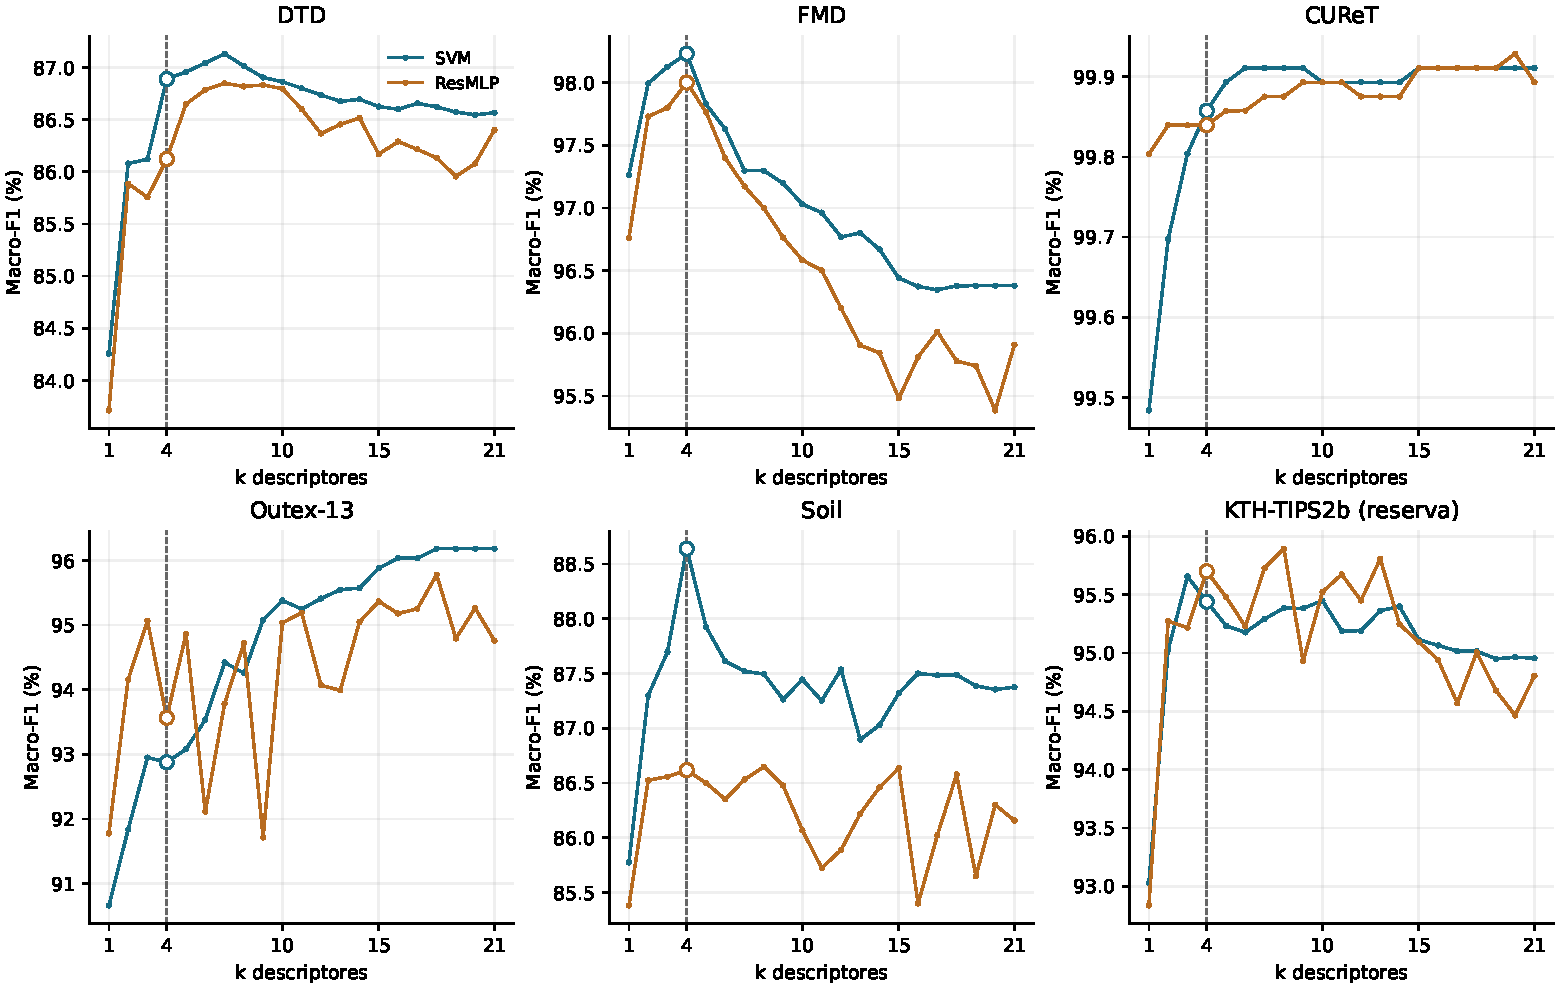
\includegraphics[width=\textwidth]{generated_topk_progression/curvas_por_dataset.pdf}
\caption[Barrido de tamaños en los seis datasets.]{Barrido de tamaños en los seis datasets. Cada panel muestra SVM y ResMLP con medias de las condiciones del dataset. La línea vertical y los círculos abiertos señalan cuatro. Las escalas verticales se ajustan por panel para mostrar las variaciones; KTH mantiene su reserva de procedencia.}
\label{fig:tm-per-dataset-curves}
\end{figure}

\section{Qué aportan N-gramas y las ampliaciones de biblioteca}
Las tablas previas distinguen 21 bloques sin N-gramas de la biblioteca de 22. El control histórico emparejado de 20 frente a 21 con N-gramas examina otra ampliación, anterior a BEiT-v2. Se conserva en la Tabla~\ref{tab:ngram-svm} para SVM y en el Anexo~\ref{app:resultados-adicionales} para ResMLP.

\begin{resulttable}
\centering\fontsize{9}{11}\selectfont\setlength{\tabcolsep}{3.6pt}
\caption{Comparación completa con SVM: medias con 20 frente a 21 bloques, incluyendo RGB Pixel N-grams + SVD. Mismas 28 condiciones externas: DTD (10), FMD (15), CUReT (2) y Outex (1). La selección se repite dentro del entrenamiento.}
\label{tab:ngram-svm}
\begin{tabular}{@{}llrrrr@{}}
\toprule
Dataset & Estrategia & F1 (20) & F1 (21) & $\Delta$ F1 & Exactitud (21) \\
\midrule
DTD & Individual & $0{,}8426$ & $0{,}8426$ & $0{,}0000\,\pm\,0{,}0000$ & $0{,}8448$ \\
DTD & Completa & $0{,}8648$ & $0{,}8629$ & $-0{,}0019\,\pm\,0{,}0026$ & $0{,}8644$ \\
DTD & Top-$k$ & $0{,}8684$ & $0{,}8684$ & $0{,}0000\,\pm\,0{,}0000$ & $0{,}8697$ \\
DTD & GFS & $0{,}8694$ & $0{,}8694$ & $0{,}0000\,\pm\,0{,}0000$ & $0{,}8707$ \\
DTD & Homogénea & $0{,}8606$ & $0{,}8606$ & $0{,}0000\,\pm\,0{,}0000$ & $0{,}8623$ \\
FMD & Individual & $0{,}9726$ & $0{,}9726$ & $0{,}0000\,\pm\,0{,}0000$ & $0{,}9727$ \\
FMD & Completa & $0{,}9644$ & $0{,}9644$ & $0{,}0000\,\pm\,0{,}0033$ & $0{,}9643$ \\
FMD & Top-$k$ & $0{,}9820$ & $0{,}9820$ & $0{,}0000\,\pm\,0{,}0000$ & $0{,}9820$ \\
FMD & GFS & $0{,}9766$ & $0{,}9766$ & $0{,}0000\,\pm\,0{,}0000$ & $0{,}9767$ \\
FMD & Homogénea & $0{,}9789$ & $0{,}9789$ & $0{,}0000\,\pm\,0{,}0000$ & $0{,}9790$ \\
CUReT & Individual & $0{,}9948$ & $0{,}9948$ & $0{,}0000\,\pm\,0{,}0000$ & $0{,}9948$ \\
CUReT & Completa & $0{,}9991$ & $0{,}9989$ & $-0{,}0002\,\pm\,0{,}0002$ & $0{,}9989$ \\
CUReT & Top-$k$ & $0{,}9989$ & $0{,}9989$ & $0{,}0000\,\pm\,0{,}0000$ & $0{,}9989$ \\
CUReT & GFS & $0{,}9988$ & $0{,}9988$ & $0{,}0000\,\pm\,0{,}0000$ & $0{,}9988$ \\
CUReT & Homogénea & $0{,}9989$ & $0{,}9989$ & $0{,}0000\,\pm\,0{,}0000$ & $0{,}9989$ \\
Outex & Individual & $0{,}9066$ & $0{,}9066$ & $0{,}0000$ & $0{,}9103$ \\
Outex & Completa & $0{,}9572$ & $0{,}9674$ & $0{,}0102$ & $0{,}9676$ \\
Outex & Top-$k$ & $0{,}9503$ & $0{,}9441$ & $-0{,}0062$ & $0{,}9456$ \\
Outex & GFS & $0{,}9426$ & $0{,}9610$ & $0{,}0184$ & $0{,}9618$ \\
Outex & Homogénea & $0{,}9307$ & $0{,}9307$ & $0{,}0000$ & $0{,}9324$ \\
\bottomrule
\end{tabular}
\par\smallskip{\footnotesize F1 designa macro-F1. $\Delta$ es la media de las diferencias pareadas (21 menos 20), acompañada de su desviación estándar cuando hay más de una partición; no es un intervalo de confianza ni una prueba de significancia.}
\end{resulttable}
\FloatBarrier


En ese control, añadir N-gramas a Completa en Outex cambia el macro-F1 de aproximadamente 0,9572 a 0,9674. La ampliación también puede cambiar qué subconjunto elige GFS o el Top-\(k\) de tamaño heredado. En DTD, Completa no mejora con la incorporación del bloque. El aporte no es uniforme y el resultado de una ampliación no se extrapola a todas las bibliotecas.

El ranking individual y la complementariedad responden preguntas distintas. La ausencia de N-gramas entre cuatro bloques mejor puntuados individualmente no demuestra que su combinación con ellos no sea útil. La tesis no presenta como ejecutado un control Top-4 más N-gramas que no tenga evidencia emparejada y cobertura identificada.

\section{Comparación externa de Top-4 en llamadas online}\label{sec:resultados-panel-online-sota}
Las Tablas~\ref{tab:tm-externos-f1} y~\ref{tab:tm-externos-ms} extraen Top-4/SVM del panel físico auditado y lo comparan con las adaptaciones externas sobre las mismas imágenes de cada condición. Las métricas de cada método se reconstruyeron con predicción y tiempo de las mismas llamadas. No se reutiliza aquí el F1 del barrido histórico con un tiempo medido después.

\begin{table}[!htbp]\centering
\fontsize{8}{10}\selectfont\setlength{\tabcolsep}{4pt}
\caption{Macro-F1 de Top-4/SVM y adaptaciones externas en el panel online auditado.}\label{tab:tm-externos-f1}
\begin{tabular}{@{}lrrrrr@{}}\toprule
Dataset & Top-4 & Neshov & HyTex & CellNN & DeepLumina\\\midrule
DTD & 0,8689 & 0,8020 & 0,6242 & 0,2162 & incompleto\\
FMD & 0,9823 & 0,9421 & 0,7414 & 0,2477 & 0,8559$^\dagger$\\
CUReT & 0,9986 & 0,9940 & 0,9831 & 0,6934 & 0,9881$^\dagger$\\
Outex-13 & 0,9288 & 0,9193 & 0,8927 & 0,6356 & 0,9073$^\dagger$\\
Soil & 0,8594 & 0,8631 & 0,7880 & 0,3550 & 0,8050$^\dagger$\\
KTH-TIPS2b & 0,9544 & 0,9245 & 0,8259 & 0,5750 & 0,8744$^\dagger$\\
\bottomrule\end{tabular}
\par\smallskip\begin{minipage}{0.98\textwidth}\footnotesize $^\dagger$ DeepLumina conserva avisos de no convergencia; DTD no tiene media completa. Los tiempos de métodos distintos provienen de fechas/estados de hardware diferentes y son descriptivos. KTH y DTD conservan sus reservas físicas/protocolares.\end{minipage}
\end{table}

\begin{table}[!htbp]\centering
\fontsize{8}{10}\selectfont\setlength{\tabcolsep}{4pt}
\caption{Latencia media observada por imagen (ms) de las mismas llamadas que sustentan la tabla de macro-F1.}\label{tab:tm-externos-ms}
\begin{tabular}{@{}lrrrrr@{}}\toprule
Dataset & Top-4 & Neshov & HyTex & CellNN & DeepLumina\\\midrule
DTD & 333,98 & 16,79 & 33,51 & 31,52 & incompleto\\
FMD & 268,96 & 16,89 & 31,18 & 29,66 & 53,33$^\dagger$\\
CUReT & 270,69 & 14,27 & 32,41 & 31,02 & 53,00$^\dagger$\\
Outex-13 & 265,38 & 14,61 & 29,04 & 29,91 & 53,54$^\dagger$\\
Soil & 70,98 & 19,17 & 33,11 & 32,98 & 57,80$^\dagger$\\
KTH-TIPS2b & 260,38 & 16,48 & 30,98 & 31,94 & 51,57$^\dagger$\\
\bottomrule\end{tabular}
\par\smallskip\begin{minipage}{0.98\textwidth}\footnotesize $^\dagger$ DeepLumina conserva avisos de no convergencia; DTD no tiene media completa. Los tiempos de métodos distintos provienen de fechas/estados de hardware diferentes y son descriptivos. KTH y DTD conservan sus reservas físicas/protocolares.\end{minipage}
\end{table}


En FMD, Top-4 alcanza aproximadamente 0,98230 frente a 0,94213 de la adaptación Neshov con MLP. Requiere más tiempo en las mediciones observadas. En Soil, Top-4 queda en 0,85940 frente a 0,86310 de Neshov, y su media temporal es mayor. Este caso desfavorable se conserva. Las mediciones de fechas distintas describen el archivo disponible y no identifican por sí solas una ventaja temporal causal.

Los valores Top-4 del panel online no se presentan como reproducción exacta de toda fila del barrido. Por ejemplo, Soil/SVM registra aproximadamente 0,88639 en el archivo de tamaños y 0,85940 en este panel. La discrepancia entre archivos requiere trazabilidad de selección, representación y ajuste; no se atribuye a una causa no demostrada ni se escoge el mayor número para una tabla final. Las conclusiones del barrido y las comparaciones por llamadas se mantienen dentro de sus archivos.

DeepLumina conserva una reserva científica: las 46 condiciones terminadas contienen avisos de no convergencia y la inspección de modelos encontró 1.653 de 2.441 clasificadores binarios en el límite de iteraciones. DTD contiene nueve de diez condiciones terminadas y no se informa una media completa. La existencia de predicciones no convierte esos ajustes en una réplica validada.

La aproximación separada Neshov FMD de 100 condiciones y 10.000 llamadas registra accuracy 94,22 \%, frente a 96,7 \% publicado. La diferencia no se oculta ni se transforma en un cambio de receta para forzar coincidencia. Se trata de una aproximación con diferencias de partición y entorno. Los porcentajes de otros artículos se interpretan de igual modo según sus protocolos.

\section{P2: optimización mediante activación por margen}\label{sec:resultados-cascada}
La auditoría reconstruye 27 condiciones SVM y 31.984 observaciones de prueba a partir de las predicciones guardadas. Verifica que, en todas las imágenes derivadas, el resultado condicional es el del mismo Top-\(k\) directo. Los tamaños del rescate van de uno a ocho: cinco condiciones usan cuatro. Son una evaluación de Top-\(k\) por condición, no 27 experimentos Top-4 fijo.

\begin{table}[!htbp]\centering
\fontsize{9}{11}\selectfont\setlength{\tabcolsep}{4pt}
\caption{Uso directo y activación por margen del mismo Top-k: auditoría de las 27 condiciones guardadas, SVM.}\label{tab:tm-cascada}
\begin{tabular}{@{}lrrrrr@{}}\toprule
Dataset & k observados & Directo F1 & Margen F1 & $\Delta$ F1 & Rescate \%\\\midrule
DTD & 4/5/6/7/8 & 0,8700 & 0,8700 & 0,0000 & 23,0\\
FMD & 3/4/5 & 0,9829 & 0,9840 & 0,0010 & 20,7\\
CUReT & 4/5 & 0,9989 & 0,9982 & -0,0007 & 20,0\\
Outex-13 & 8 & 0,9426 & 0,9369 & -0,0056 & 19,9\\
Soil & 3/5/6/7/8 & 0,8701 & 0,8734 & 0,0033 & 23,6\\
KTH-TIPS2b & 1/2 & 0,9400 & 0,9445 & 0,0045 & 38,2\\
\bottomrule\end{tabular}
\par\smallskip\begin{minipage}{0.98\textwidth}\footnotesize Se conserva el Top-k específico de cada condición; k no es siempre cuatro. KTH mantiene la reserva de procedencia y no integra inferencia conjunta. La tasa incluye Top-k directo cuando esa fue la ruta seleccionada.\end{minipage}
\end{table}


Se identificaron además las cinco condiciones cuyo rescate tiene cuatro bloques y coincide exactamente con el subconjunto Top-4 del barrido de esa partición. La Tabla~\ref{tab:tm-fixed4-margin} conserva sus aumentos, pérdidas y empates. El subconjunto se define por identidad de bloques y tamaño, no por favorecer la activación. No representa cobertura Top-4 por margen en los seis datasets.

\begin{table}[!htbp]\centering
\fontsize{9}{11}\selectfont\setlength{\tabcolsep}{4pt}
\caption{Condiciones donde el rescate coincide con el Top-4 del barrido, SVM.}\label{tab:tm-fixed4-margin}
\begin{tabular}{@{}lrrrr@{}}\toprule
Condición & Directo F1 & Margen F1 & $\Delta$ F1 & Rescate \%\\\midrule
DTD / split 10 & 0,860440 & 0,864968 & 0,004529 & 24,47\\
DTD / split 8 & 0,854571 & 0,853492 & -0,001079 & 22,34\\
FMD / fold 2 & 0,984994 & 0,984994 & 0,000000 & 17,00\\
FMD / fold 3 & 1,000000 & 1,000000 & 0,000000 & 19,50\\
CUReT / A a B & 0,998218 & 0,996792 & -0,001426 & 22,45\\
\bottomrule\end{tabular}
\par\smallskip\begin{minipage}{0.98\textwidth}\footnotesize Subconjunto definido por k=4 y coincidencia de bloques, no por signo del resultado. Son cinco condiciones de tres datasets; no una evaluación Top-4 por margen completa en seis datasets.\end{minipage}
\end{table}


Se selecciona cascada en 26 condiciones y uso directo en una. Las bases de las rutas condicionales son SigLIP en veinte condiciones, BEiT-v2 en cinco y ResNet-50 en una. Estas elecciones provienen del criterio interno identificado en el método; no se escoge una base por el mayor F1 externo.

En FMD, el uso directo registra macro-F1 medio 0,982926 y la política por margen 0,983953. En Outex, la política condicional baja de 0,942574 a 0,936950. CUReT presenta una pérdida pequeña; DTD queda muy próximo en promedio. Soil y el KTH histórico muestran aumentos. La compuerta no produce una mejora uniforme.

La ruta condicional puede superar a Top-\(k\) porque conserva la predicción base en las imágenes que no deriva. Top-\(k\) directo no es un techo matemático de esa combinación. Del mismo modo, un margen alto puede conservar un error que la segunda etapa habría corregido. La auditoría guarda ambos conteos, junto con los cambios de clase.

\section{Adquisición proyectada y pilotos físicos}\label{sec:resultados-gpu}
\begin{table}[!htbp]\centering
\fontsize{9}{11}\selectfont\setlength{\tabcolsep}{4pt}
\caption{Costos de extracción proyectados de las rutas históricas. No son latencias online por dataset.}\label{tab:tm-costos}
\begin{tabular}{@{}lrrr@{}}\toprule
Dataset & Directo (ms) & Margen (ms) & Reducción \%\\\midrule
DTD & 661,82 & 171,95 & 74,0\\
FMD & 583,42 & 138,74 & 76,2\\
CUReT & 655,64 & 153,45 & 76,6\\
Outex-13 & 729,48 & 165,90 & 77,3\\
Soil & 271,28 & 85,20 & 68,6\\
KTH-TIPS2b & 278,05 & 64,89 & 76,7\\
\bottomrule\end{tabular}
\par\smallskip\begin{minipage}{0.98\textwidth}\footnotesize Cociente de medias por dataset; perfiles históricos por componente. No incluye una nueva medición física ni valida las discrepancias de representación.\end{minipage}
\end{table}

\begin{figure}[!htbp]\centering
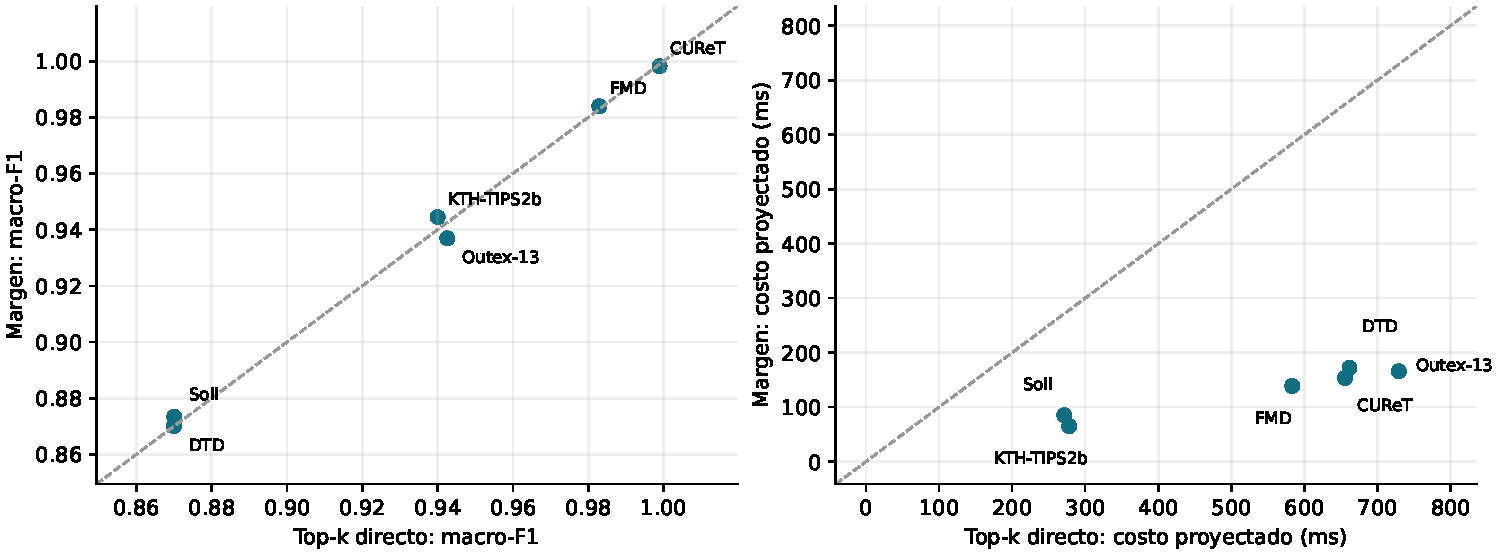
\includegraphics[width=\textwidth]{generated_topk_margin/directo_margen.pdf}
\caption{Comparación por dataset del uso directo y por margen: calidad a la izquierda y adquisición proyectada a la derecha. La diagonal indica igualdad de la magnitud; el panel de costo no es un cronometraje físico nuevo. KTH conserva su reserva.}
\label{fig:tm-direct-margin}
\end{figure}

La Tabla~\ref{tab:tm-costos} reporta \(\widehat C_V\): adquisición proyectada con la fracción externa observada después de fijar la política. La selección utilizó \(\widehat C_{\mathrm{sel}}\), calculada con las predicciones internas OOF. Que ambas tasas difieran no implica que se haya vuelto a elegir el umbral con el test. Los porcentajes describen el perfil de extracción por componentes y se mantienen separados de los cronometrajes físicos.

\begin{table}[!htbp]\centering\fontsize{8}{10}\selectfont
\caption{Piloto físico de la política con base seleccionada, una condición por dataset. Modelos residentes e imágenes decodificadas; una imagen por clase y tres repeticiones pareadas.}
\label{tab:gpu-benchmark}
\begin{tabular}{@{}lrrrrl@{}}\toprule
Dataset & Imágenes & Pares & Margen ms & Directo ms & Reserva\\\midrule
DTD & 47 & 141 & 90,57 & 295,55 & alcance del piloto\\
FMD & 10 & 30 & 13,01 & 208,08 & alcance del piloto\\
CUReT & 61 & 183 & 92,52 & 270,60 & representación\\
Outex13 & 68 & 204 & 111,47 & 354,31 & alcance del piloto\\
Soil & 7 & 21 & 41,99 & 109,10 & representación\\
KTH-TIPS2b & 11 & 33 & 46,08 & 188,33 & variante histórica\\
\bottomrule\end{tabular}
\end{table}

El piloto reúne 204 imágenes y 612 parejas, no 612 imágenes independientes. Los tiempos observados favorecen la ruta condicional en esas condiciones. Sin embargo, CUReT y Soil mantienen discrepancias entre los vectores físicos y cacheados; sus cosenos mínimos fueron aproximadamente -0,0707 y 0,0085. Coincidir en clase o ruta no demuestra identidad de representación. Los tiempos no cierran esa reserva ni acreditan reducción general en los seis conjuntos.

El control físico KTH con salida directa justa documentó también que una cascada puede ser más lenta cuando Top-\(k\) ya es barato. La posibilidad de elegir uso directo forma parte de la decisión estudiada, no constituye un caso que se deba omitir.

\section{Síntesis de evidencia}
P1 queda respaldada por un barrido amplio y por comparaciones que identifican tanto ventajas de compactar como pérdidas frente a representaciones mayores. P2 dispone de una comparación por predicciones del mismo Top-\(k\), costos analíticos y pilotos físicos delimitados. La cobertura completa de las predicciones no convierte automáticamente los costos en latencias físicas completas.

Los experimentos de ensamble y poda permiten otras preguntas y se conservan en el Anexo~\ref{app:complementarios}. No se utilizan sus porcentajes de ahorro para atribuir un resultado al Top-\(k\) directo/por margen del cuerpo principal.
